\subsection{CAIDA, RIPE Atlas, \& Measurement Lab traceroutes}[Chris M.]

The \caida, \gls{ripe} Atlas, and Measurement Lab own nodes across the world that routinely run traceroutes to different locations. 

\caida maintains what they call the Archipelago network (or just Arc), a series \textapprox{}180 of Raspberry Pi's across the world that run measurements to different parts of the internet. We're interested in their prefix probing data set, which involves running complete traceroutes to at least one host in every /24 prefix. That is, every day, every Arc node runs a traceroute that picks up on one host in 130.215.1.x address, one in 130.215.2.x, and so on. This produces an \textit{enormous} amount of data, dating back to 2014 with over 6,000 compressed binary files. We have a series of python scripts that can extract this data and shove it into either hundreds of SQLite databases, or one big PostgreSQL database for easier analysis.

\gls{ripe} Atlas and Measurement Lab run on approximately the same principle, collecting tens of thousands of traceroutes per day.

To gain a better understanding of the data from \caida we conducted some basic statistic analyses to gauge the spread of the data. The charts below were created using about a sixth of the data available, with only source to final destination routes considered -- effectively just a ping.

\begin{figure}[H]
    \centering
    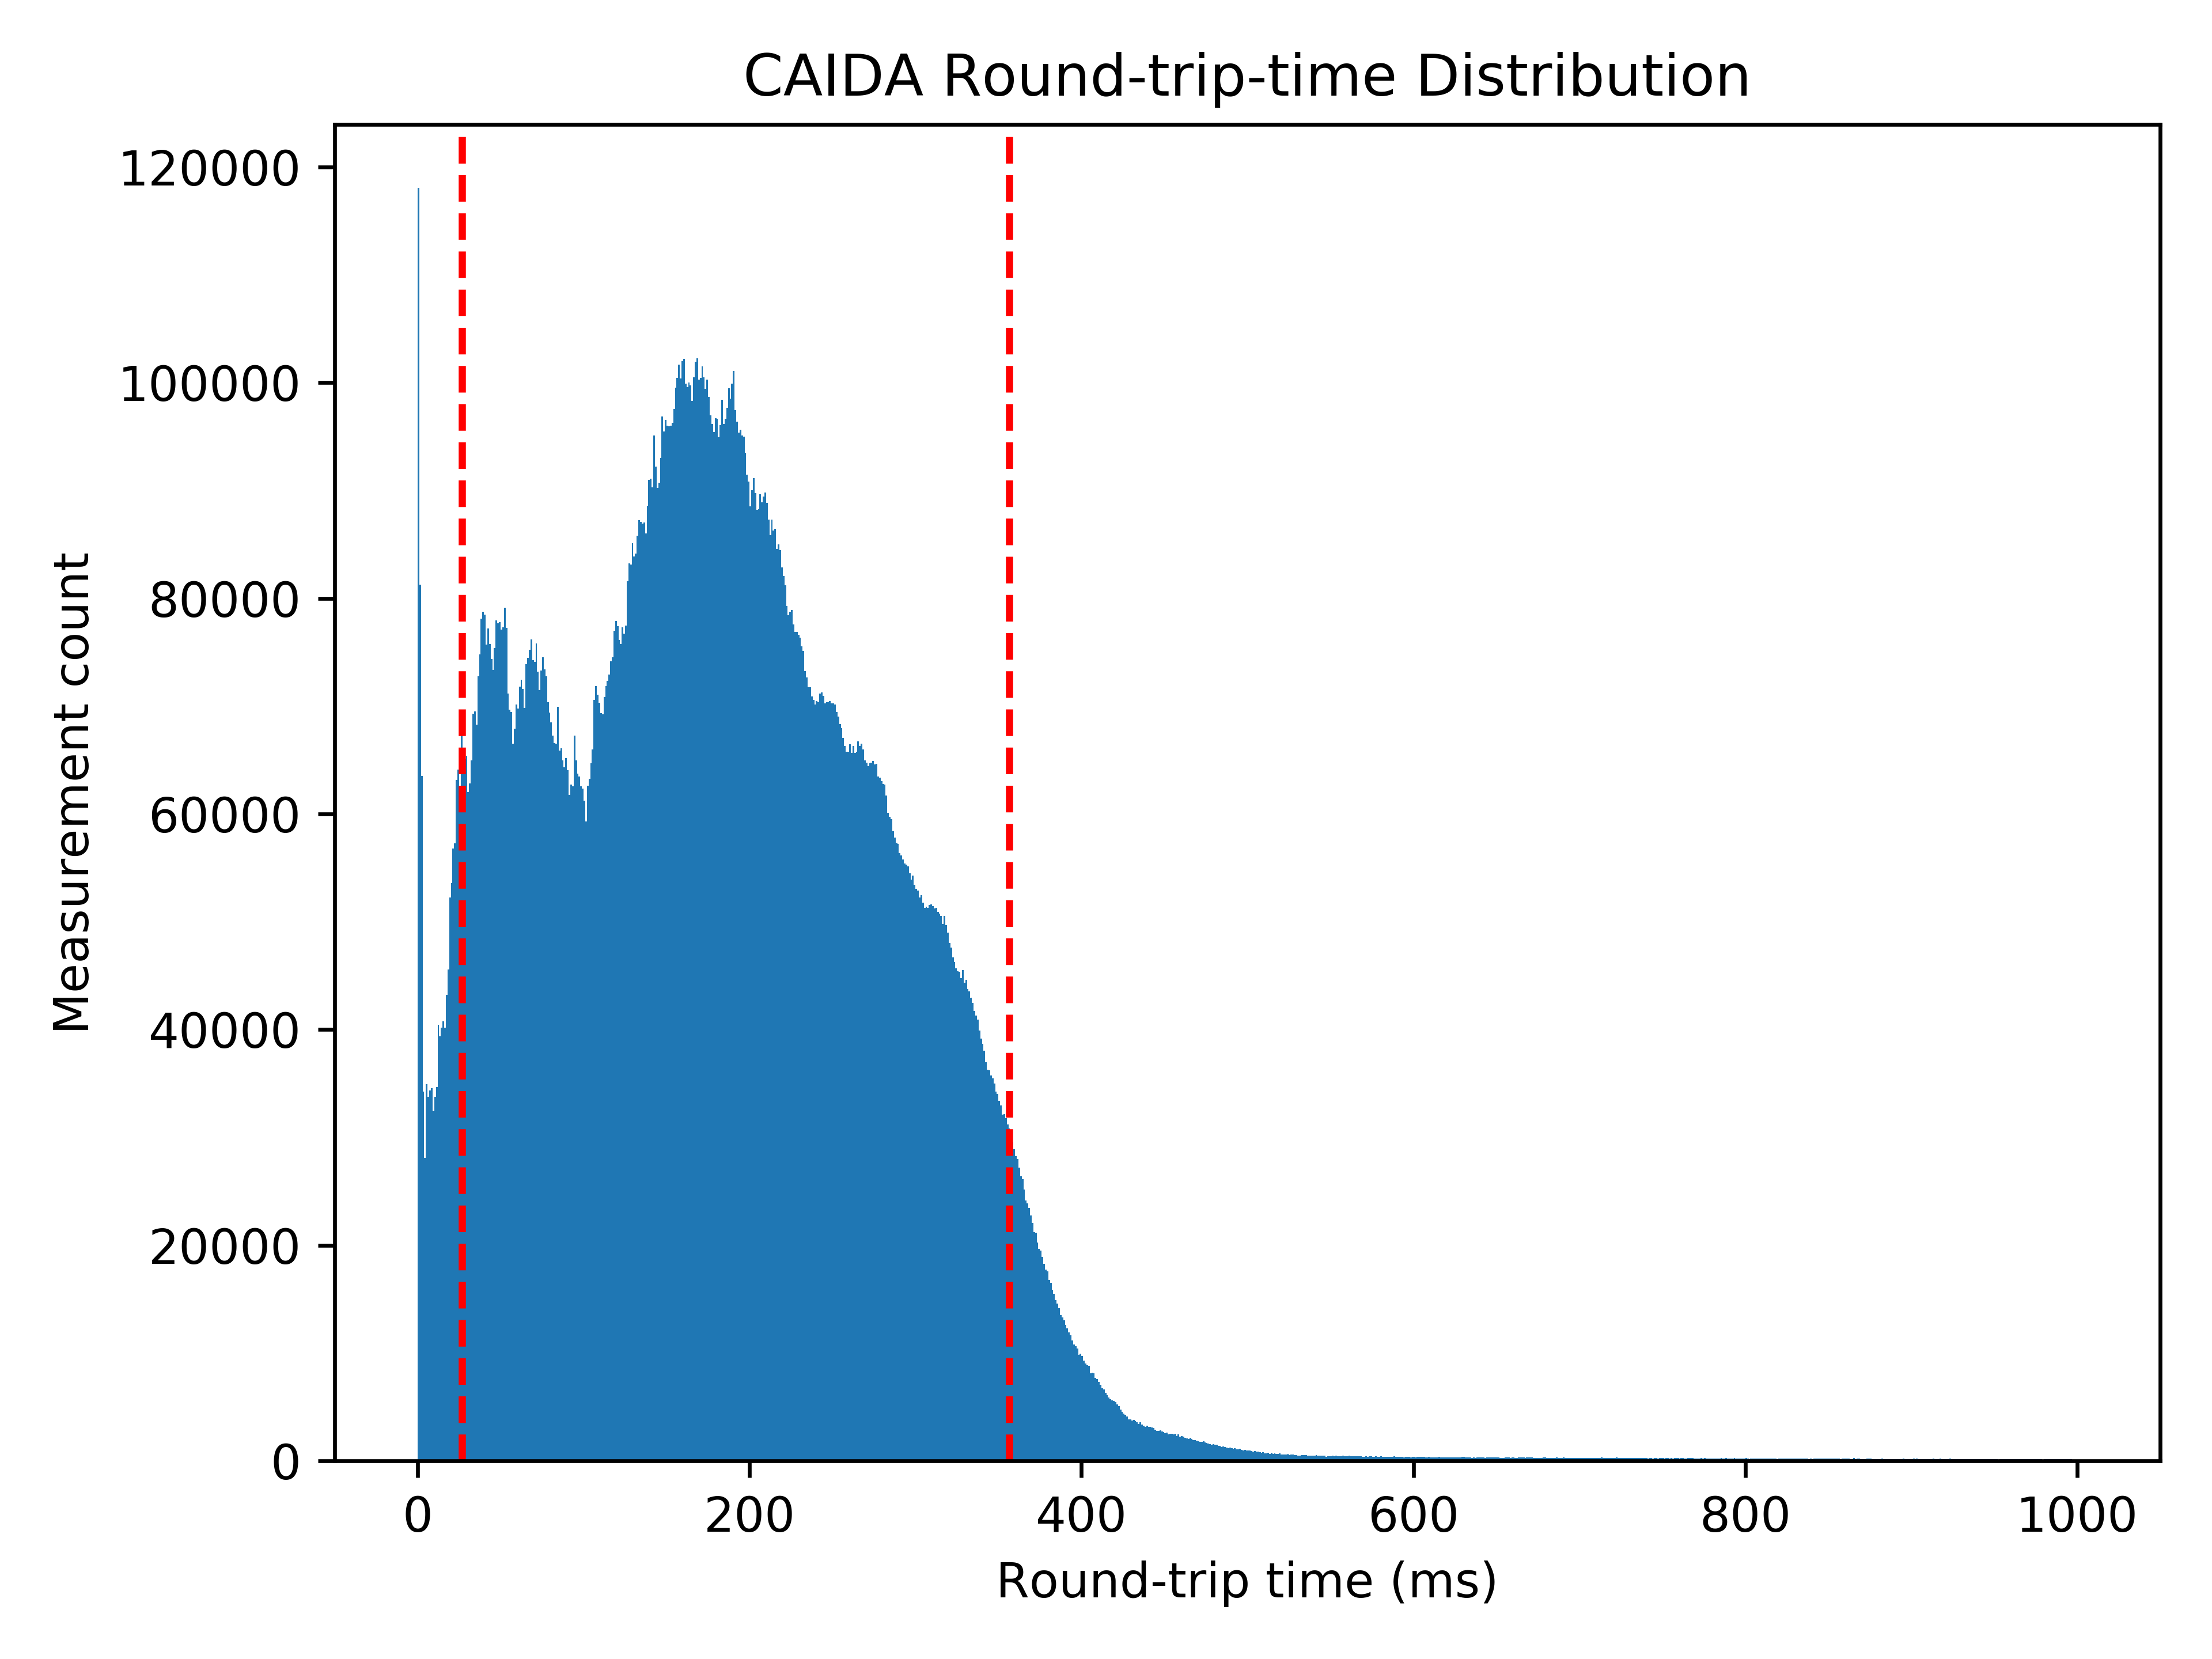
\includegraphics[width=\textwidth]{CAIDA_rtt_dist.png}
    \caption{Distribution of CAIDA RTTs with 5th and 95th percentiles shown}
    \label{fig:rtt_dist}
\end{figure}

Figure \ref{fig:rtt_dist} shows the distribution of \rtts recorded by CAIDA, with extreme values above 1000 ms omitted. The graph shows a reasonably sharp peak with a curious bimodal distribution. Fortunately, this easily explainable -- the two peaks likely represent sources from different landmasses. For instance, the larger peak on the right might correspond to hosts in Europe and Asia, while the smaller peak on the left might correspond to North and South America.

\begin{figure}[H]
    \centering
    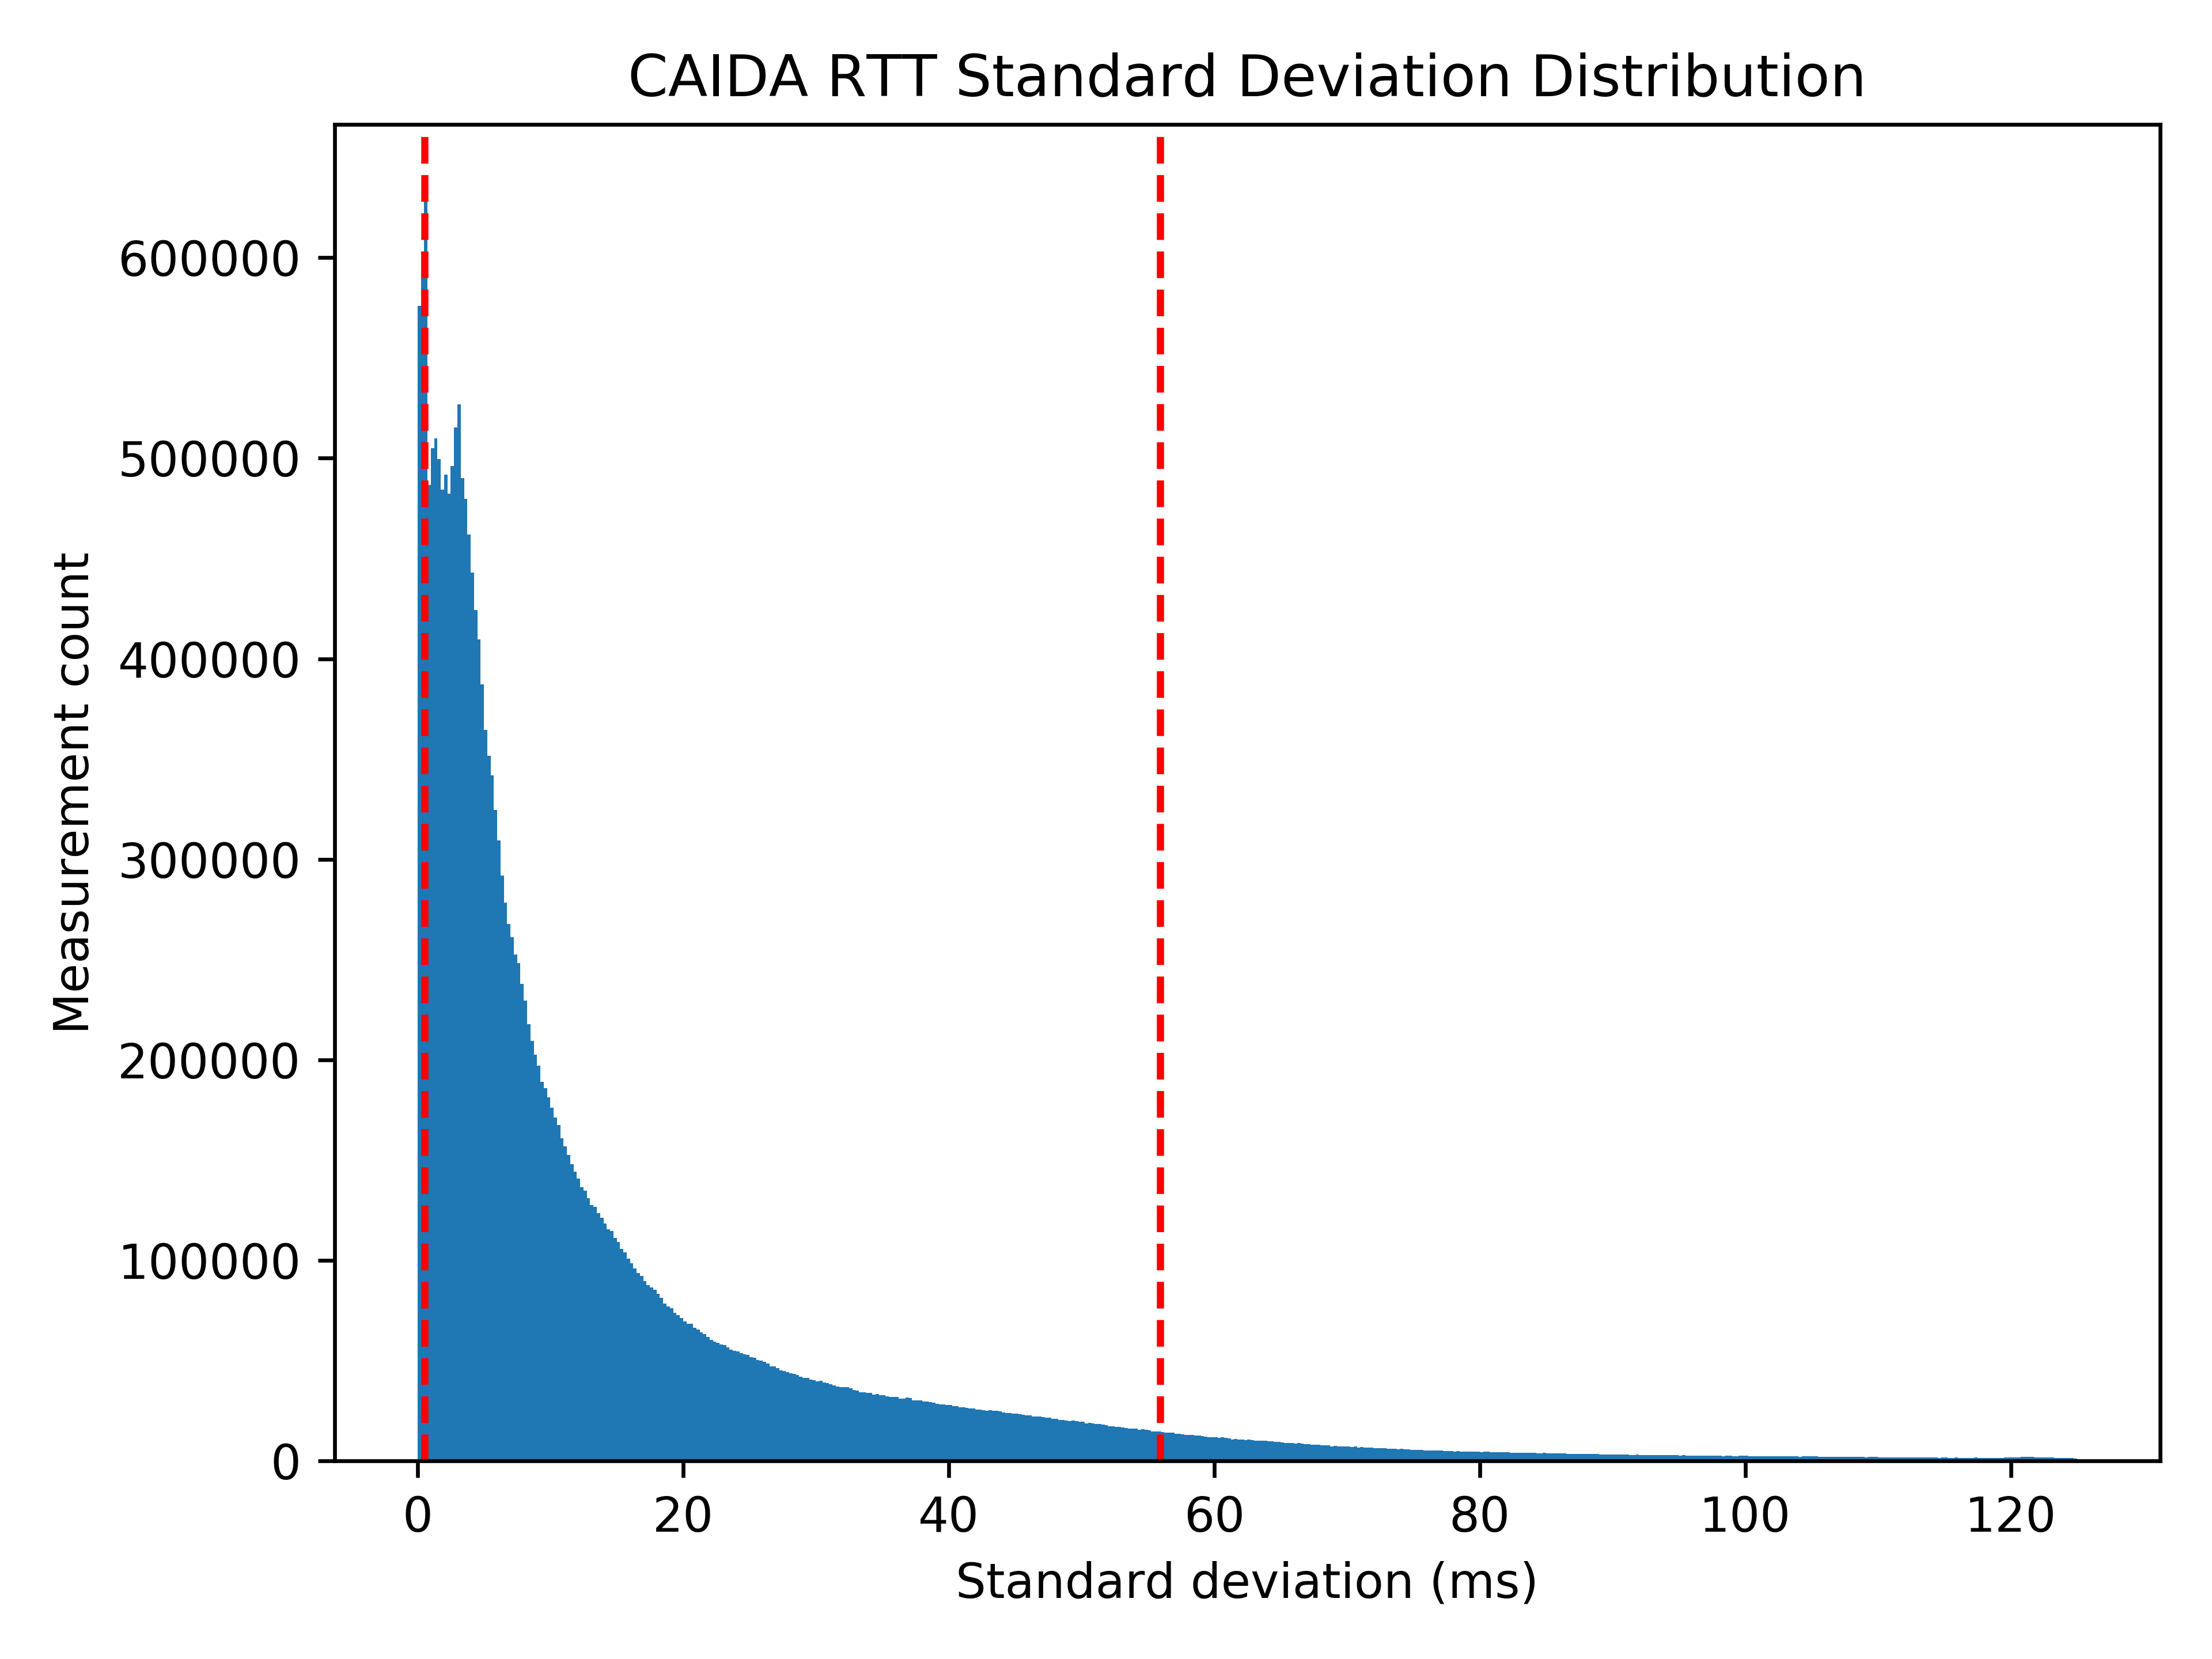
\includegraphics[width=\textwidth]{CAIDA_rtt_stdev_dist.png}
    \caption{Distribution of CAIDA RTT standard deviations with 5th and 95th percentiles}
    \label{fig:rtt_stdev_dist}
\end{figure}

Since \caida reports many trials per source-destination pair, a measure of the standard deviations of those measurements is useful to gauge jitter along connections. Figure \ref{fig:rtt_stdev_dist} shows the distribution of standard deviations, which shows a beautifully sloped curve that peaks on the left -- lower standard deviation means lower spread of data, so we can reasonably infer the data is of high quality.

\begin{figure}[H]
    \centering
    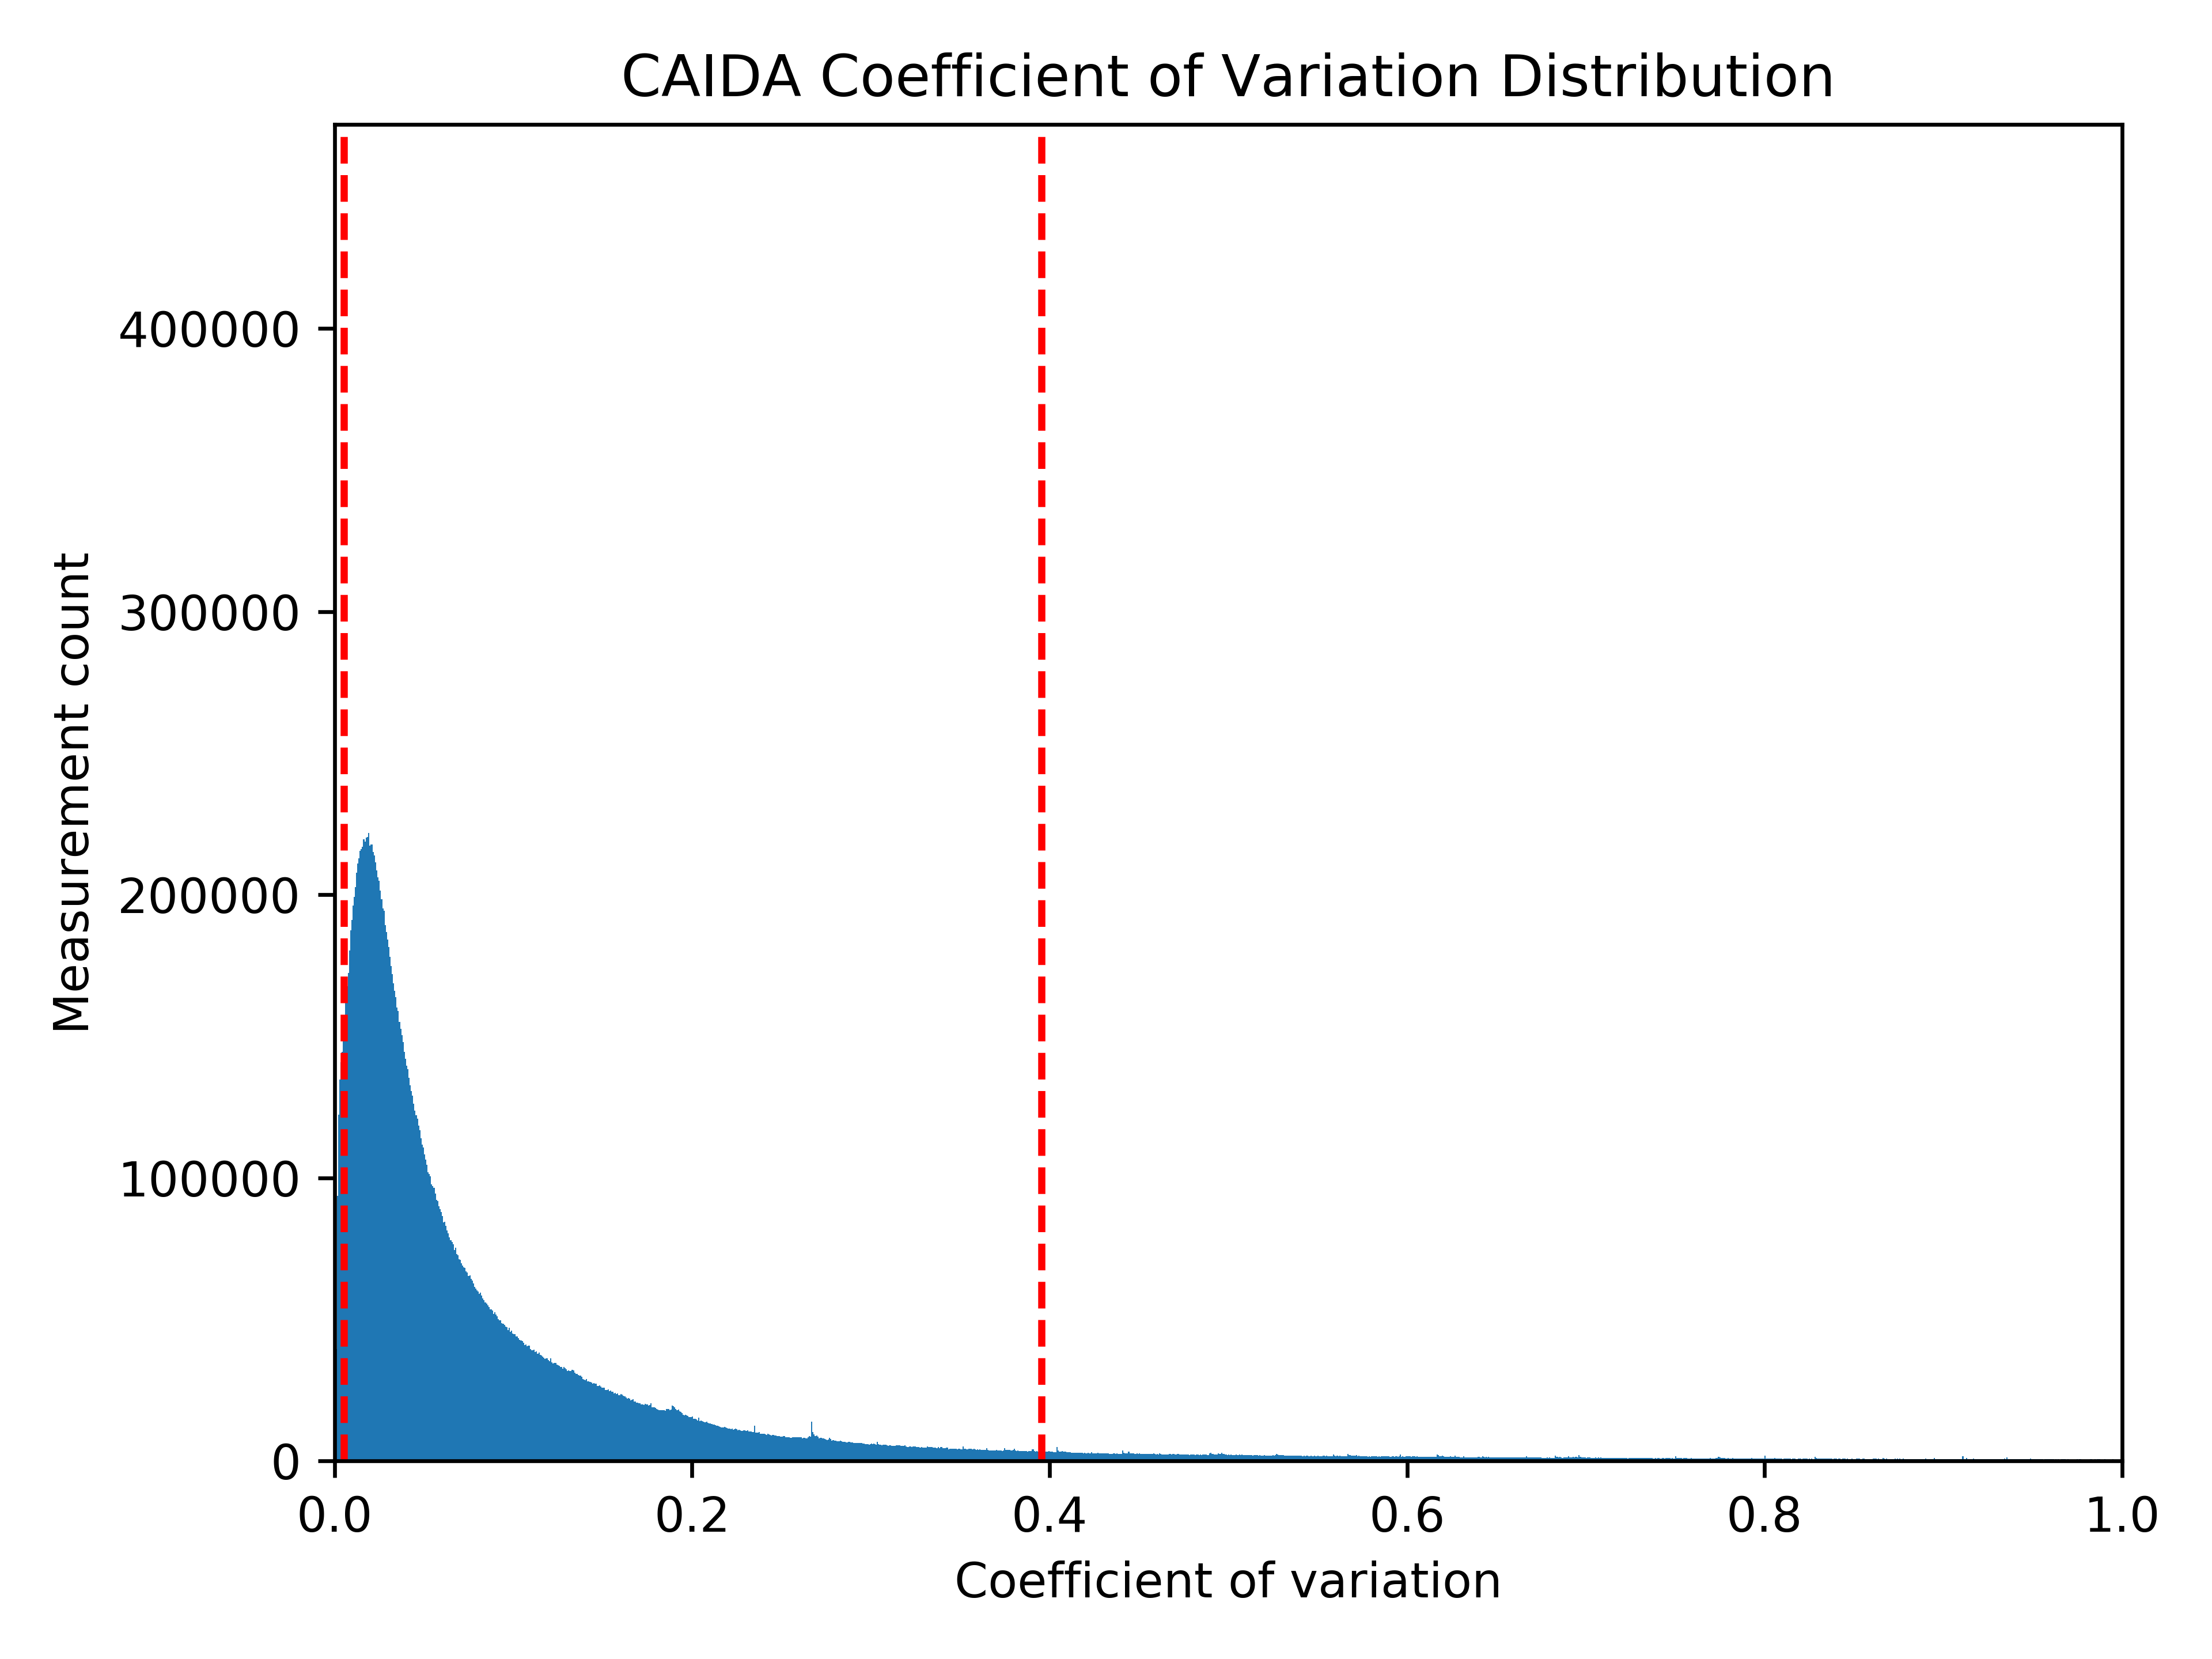
\includegraphics[width=\textwidth]{CAIDA_cv_dist.png}
    \caption{Distribution of CAIDA RTT coefficients of variance with 5th and 95th percentiles} 
    \label{fig:rtt_cv_dst}
\end{figure}

To compound on that, figure \ref{fig:rtt_cv_dst} shows a distribution the \glspl{cv} for the data set, dimensionless values that can be interpreted the same regardless of the underlying data. These are calculated by dividing the standard deviation by the mean, so lower is better. Broadly speaking the majority of the data is of excellent quality, but this information is definitely useful on setting appropriate limits for filtering.

\subsubsection{Raw RTT}
Combined, these three data sets give us access to huge amounts of data on the \rtts between nodes everywhere in the world -- hundreds of millions of machines -- both for end-to-end connections and connections to intermediaries. Since there are many traceroutes for each source-destination pair, we can control for jitter by averaging measurements together and reporting on other common statistics values (range, standard deviation, etc).

Each \ip in the data set can be geo-located to provide us with reasonably accurate locations for every \ip that appears in the dataset. These locations plus the \rtts can be used to build a heat map that shows what average \rtt looks like from any given location in the US. Filtering can be done to further refine this, e.g. average \rtt to only US servers, only international servers, and so on.

\subsubsection{RTT per distance}
\rtts naturally vary with distance, both because the number of nodes in the path tends to increase with path length (increasing routing delays) and because time to get data from point A to point B is governed by the speed of light. The amount an \rtt varies with distance, though, depends on the quality of the infrastructure between connection endpoints, so \rtt divided by distance (in units of ms/km) is a good metric for understanding internet connectivity.

To that that end we've conducted some early data analysis using a subset of the \caida prefix probing dataset, and have generated the following heatmap:

\begin{figure}[H]
    \centering
    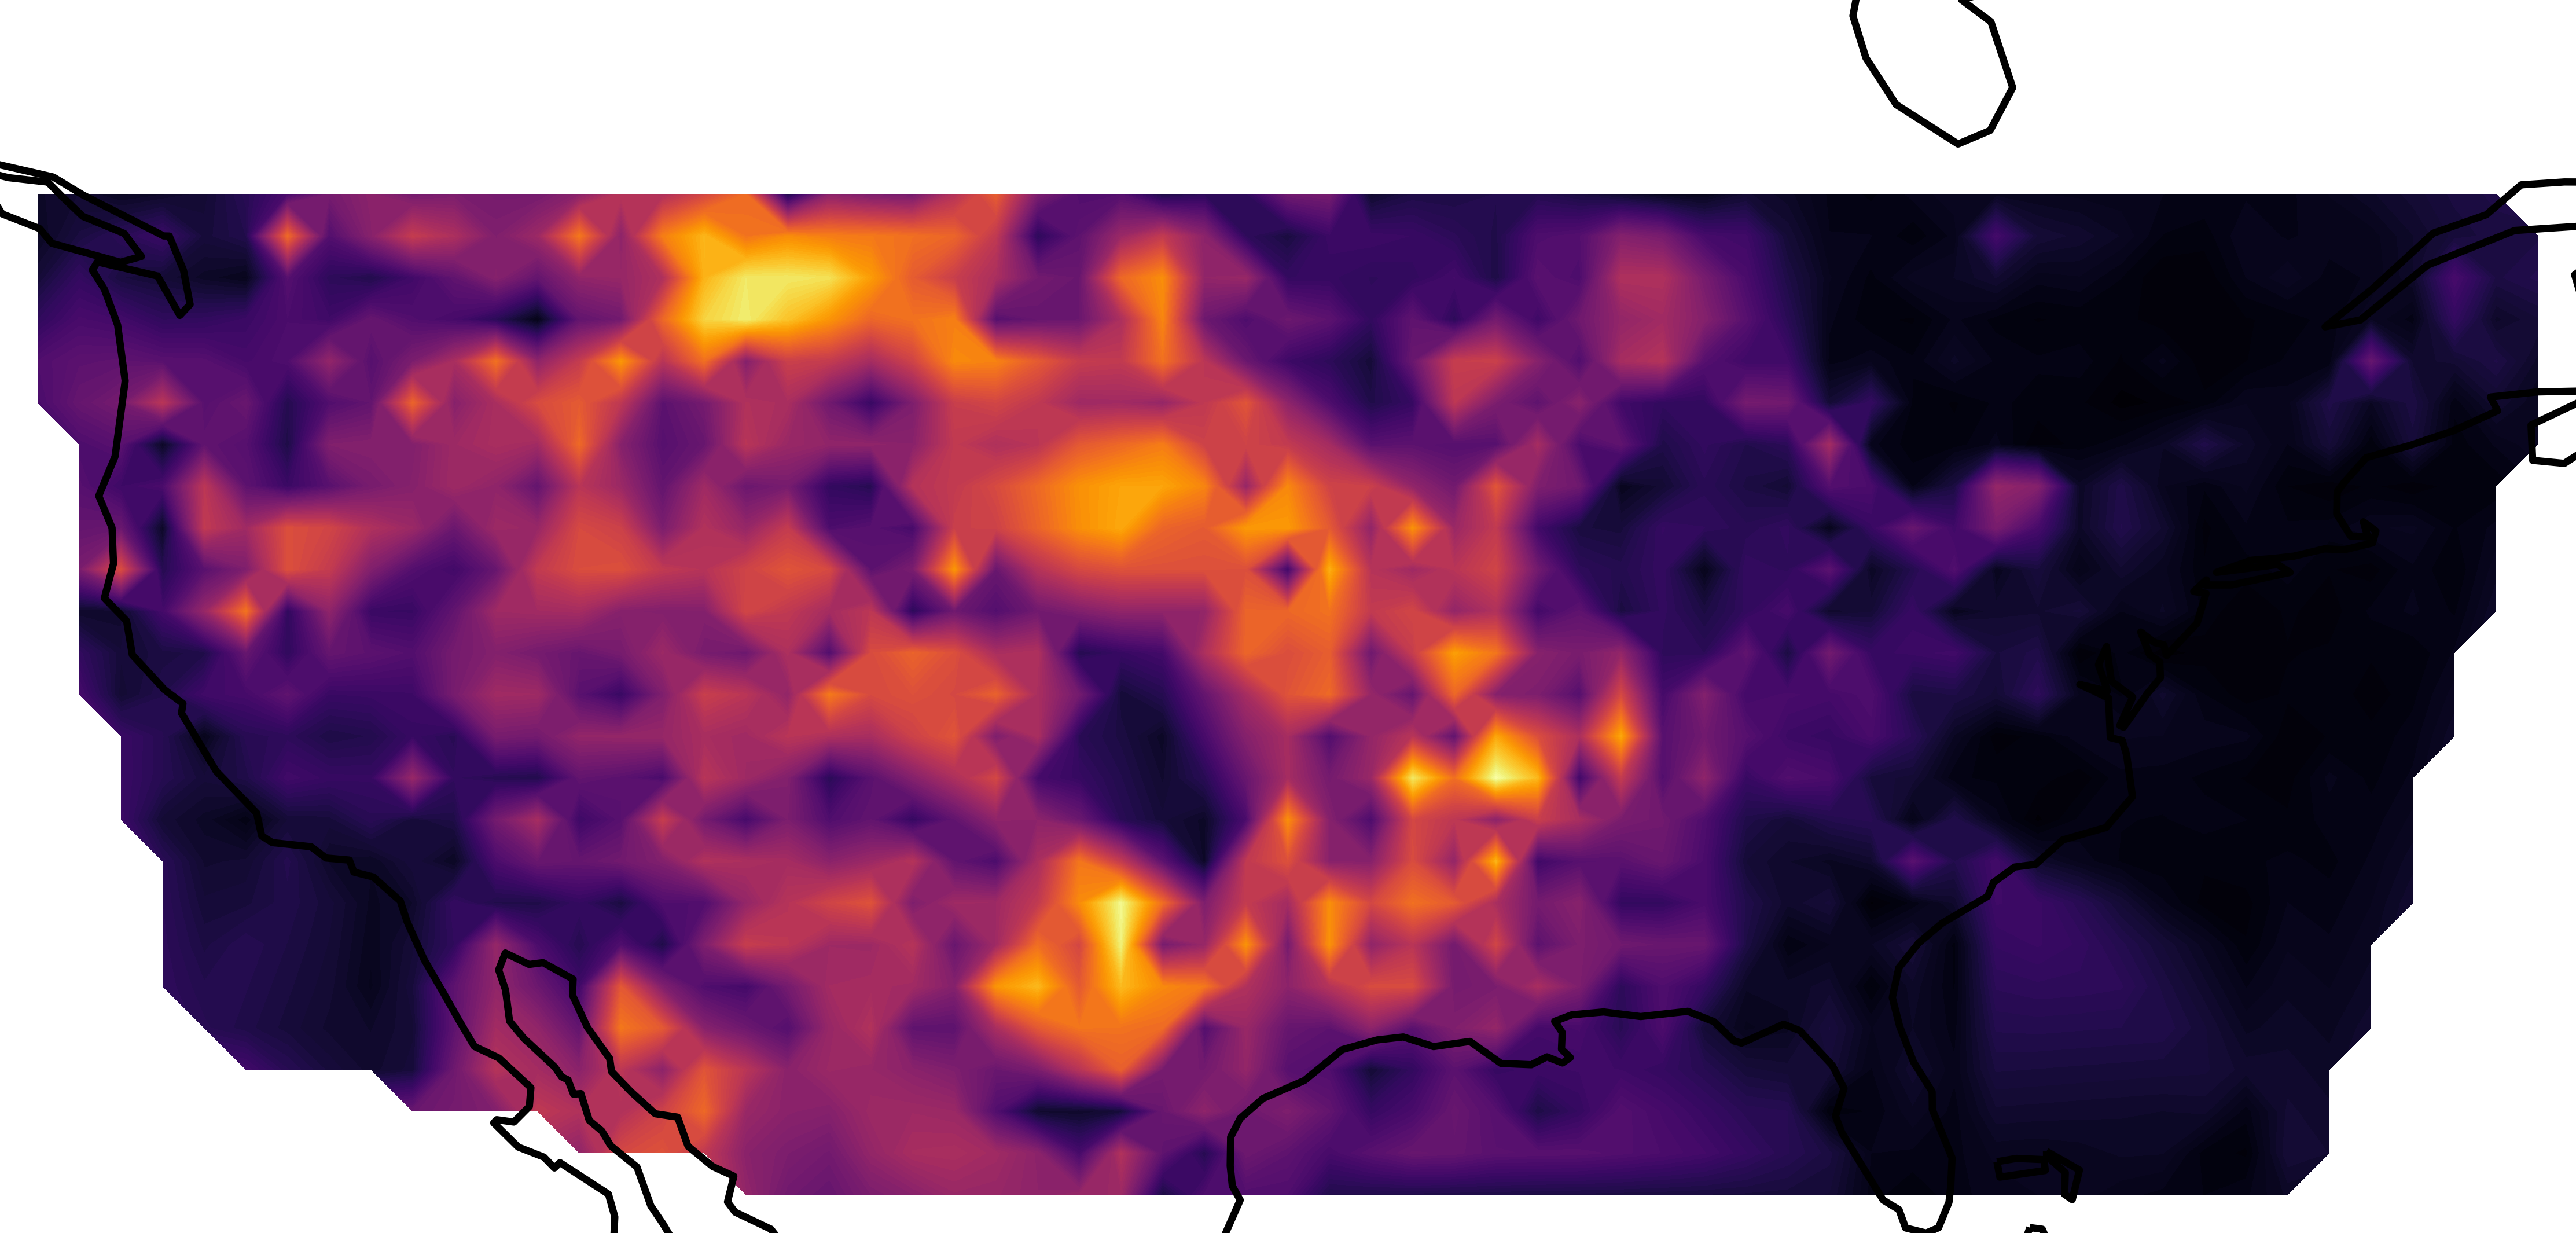
\includegraphics[width=\textwidth]{CAIDA_connect_heatmap.png}
    \caption{Heatmap of ms/km values}
    \label{fig:caida_connectivity_heatmap}
\end{figure}

Figure \ref{fig:caida_connectivity_heatmap} shows a heatmap of connectivity across the US where brighter areas correspond to lower internet connectivity. This roughly corresponds to data available from \isps, which indicate that the Northwest, for instance, generally has much poorer internet access. This map was generated using python matplotlib and some data analysis techniques to reduce the sheer quantity of data from hundreds of millions of data points to only a few thousand (see \S{}\ref{sec:optimization}).

\begin{figure}[H]
    \centering
    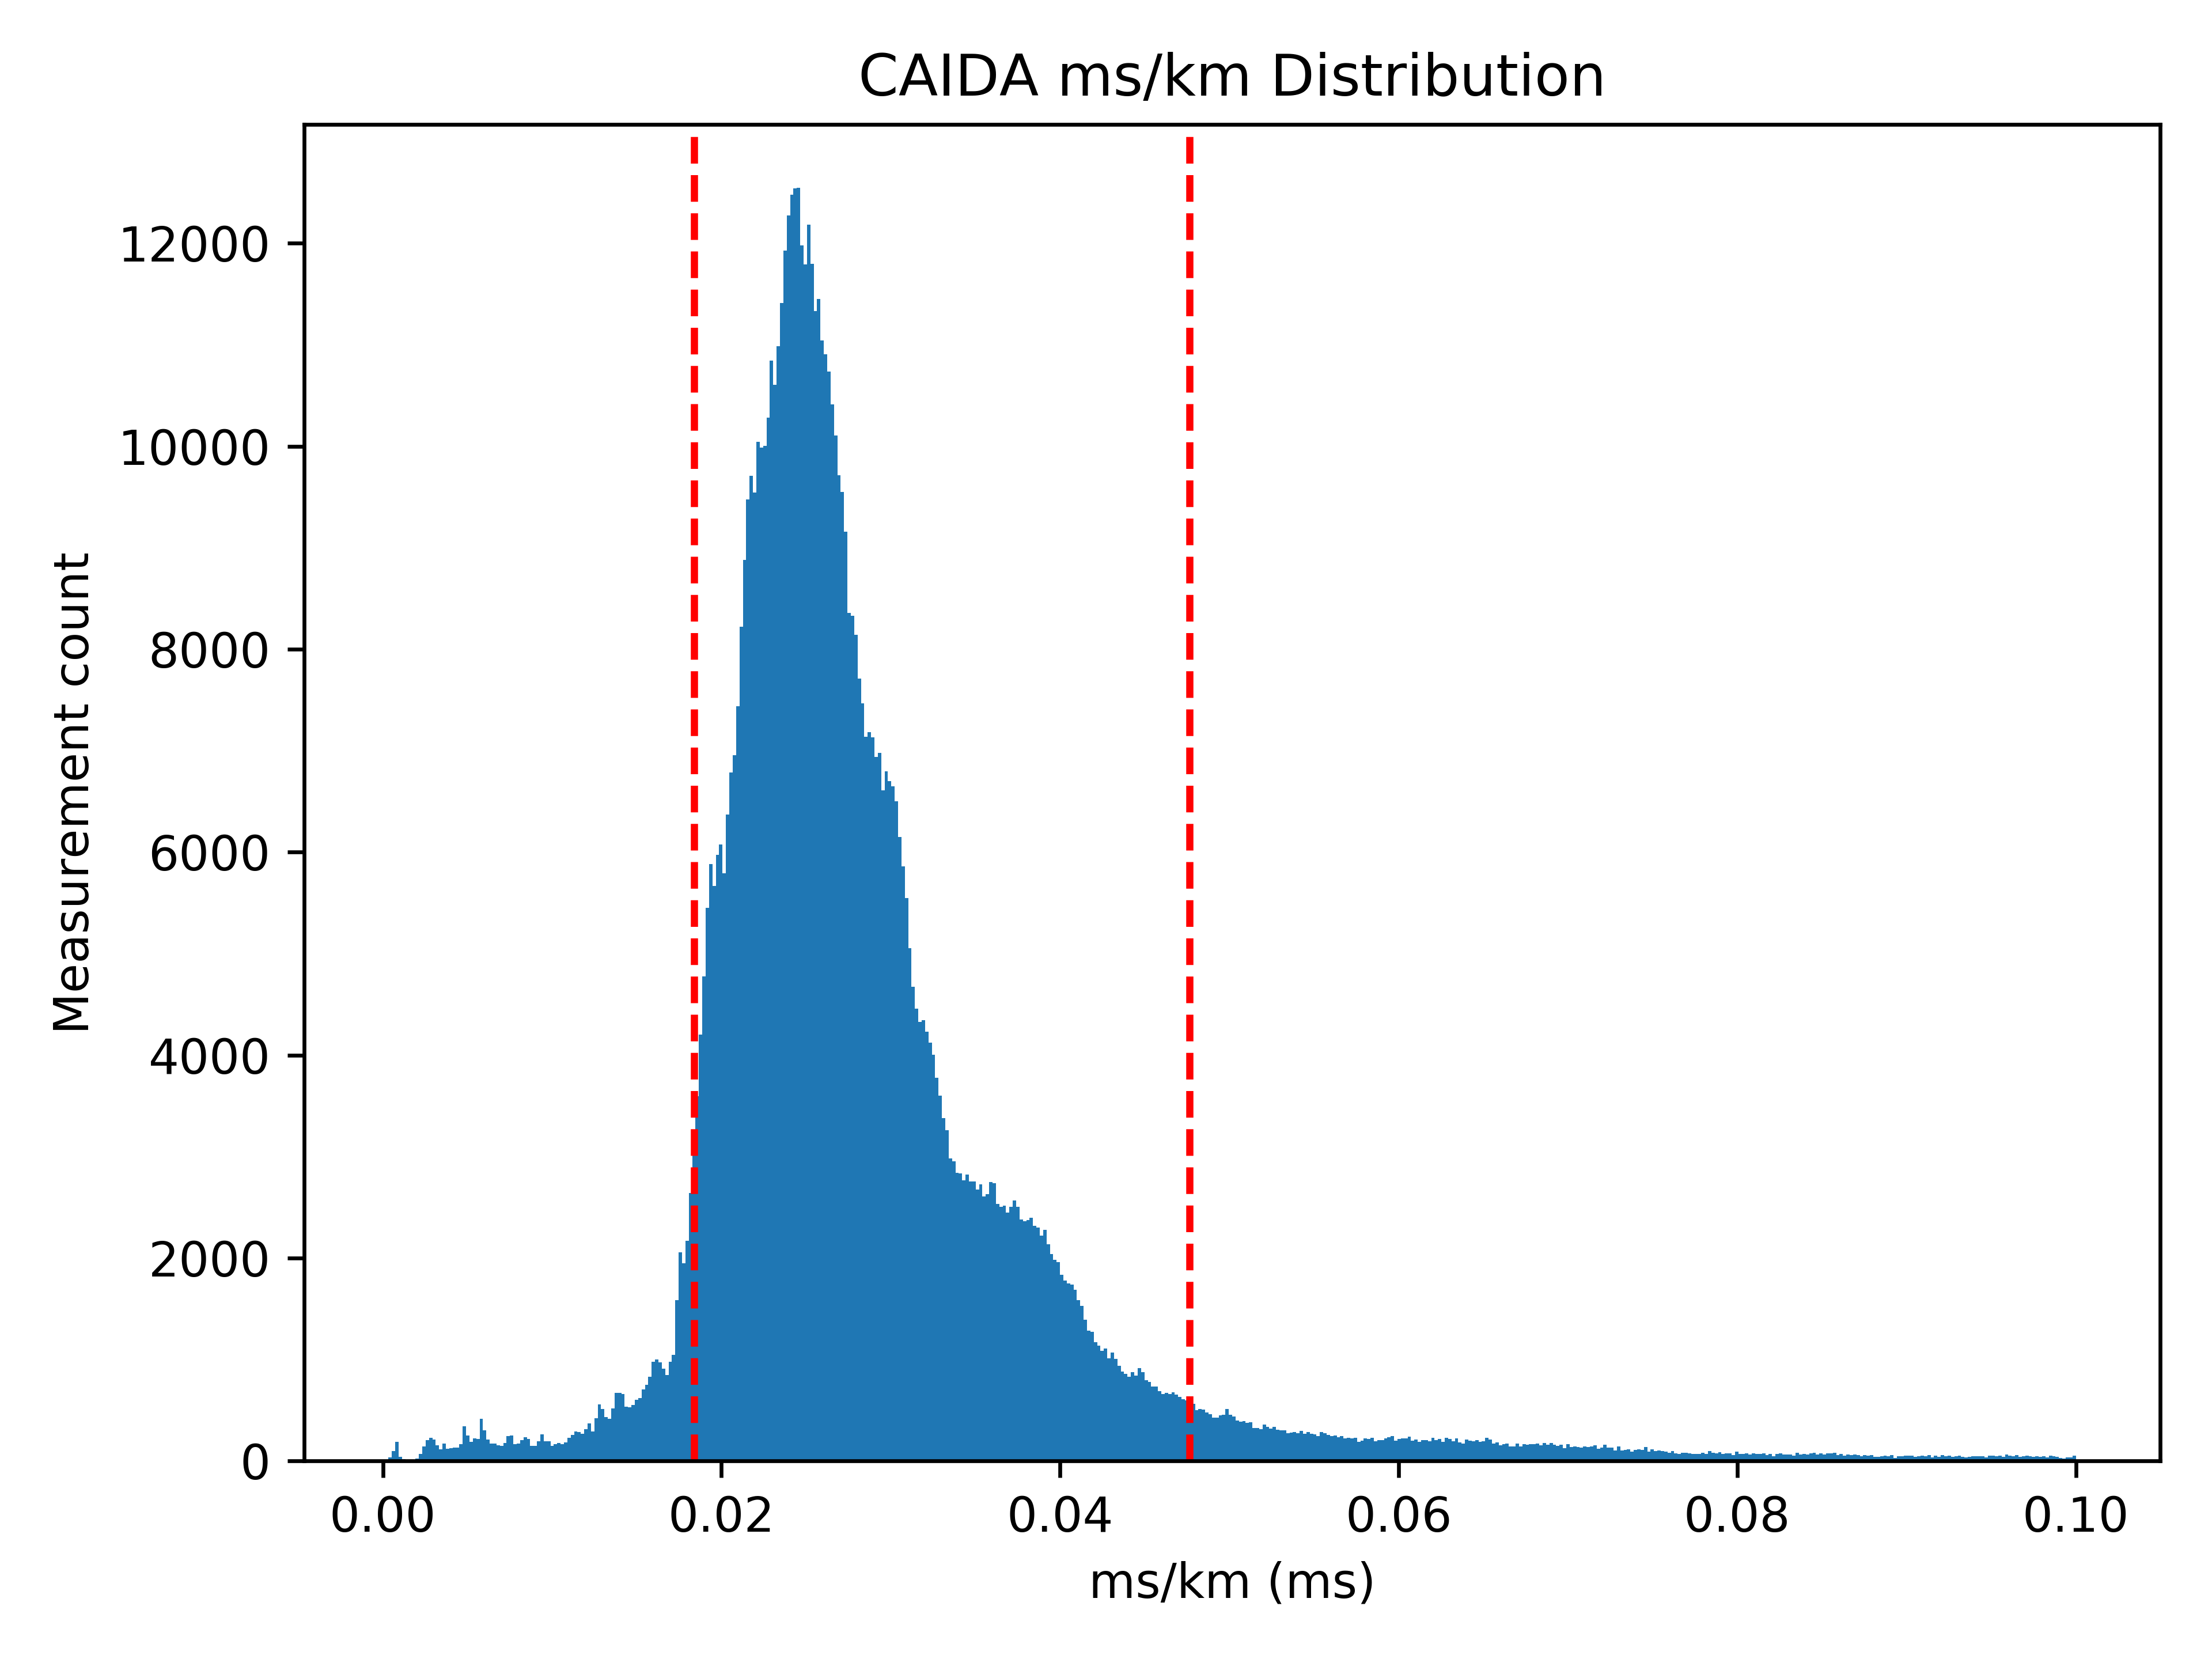
\includegraphics[width=\textwidth]{CAIDA_connect_dist.png}
    \caption{Distribution of CAIDA ms/km values with 5th and 95th percentiles}
    \label{fig:caida_connectivity_dist}
\end{figure}

Figure \ref{fig:caida_connectivity_dist} shows is based on the data as figure \ref{fig:caida_connectivity_heatmap}, but shows a distribution instead. This is another fairly narrow peak, but with enough interesting variation and shoulders to hint at underlying patterns and data worth analyzing.

\subsubsection{Backbone analysis}

The benefit to collecting traceroutes instead of direct pings is that we obtain an ordered list of all nodes between endpoints. This forms a simple linear directed graph for each traceroute; by finding common source/destination pairs between traceroutes we can add to the graph. Series of pairs that are very commonly traveled can be automatically inferred to be backbone connections that great portions of traffic travels through. By identifying these nodes we can extract information on how long it takes each node in the graph to reach the nearest identified backbone node. This should provide useful insight on internet connectivity, since connection speed to the nearest major internet exchange likely has a much greater influence on connectivity than does the ability of a given node to connect to any other node.

\subsubsection{Direct RTT, route RTT, \& calculated hop RTT}

For each traceroute there are three modes of analysis: direct ping, all pings, and hop ping calcuation. A direct ping just means discarding all intermediary hops and only considering \rtt to the target node, hence being equivalent to a direct ping. Considering all pings in a traceroute means recording \rtt to each individual node. That is, if you have $A\rightarrow B\rightarrow C\rightarrow D$, you record data for $A\leftrightarrow B, A\leftrightarrow C$, and $A\leftrightarrow D$. These in turn correspond to actual ping-equivalents received from the remote node.

Calculated hops are more complicated. For each hop along the route an \rtt value is recorded, e.g. $B=5, C=12, D=25$. By subtracting each node's \rtt from the \rtt of the node \textit{ahead} of it, we can estimate the \rtt from the first node to the second. So in this case, we would calculate $B\leftrightarrow C=7$ and $C\leftrightarrow D=13$. These values are approximate since we don't have a direct measurement, but useful all the same in calculating the quality of individual links. 

By combining the three methods, for a traceroute with $n$ hops we obtain $2n-2$ datapoints. 

\label{sec:optimization}\subsubsection{Optimization Techniques \& Database Design}

To put it mildly, there is a \textit{massive} amount of data to analyze. We estimated about 185 billion datapoints from \caida alone using one method of analysis; even if it's off by an order of magnitude or two, we're still dealing with datapoints in the billions. This amount of raw data is clearly impossible to plot all in one graph, and even if we did, the data would be minimally useful. To that end we've devised a few basic methods for reducing the size of the dataset into something more manageable, without compromising the meaning behind the data. Some of these methods are common statistics and data science techniques, some are not.

\paragraph{Grouping source-destination pairs}

We interpret multiple instances of source to destination pairs as the equivalent of multiple "trials" of an experiment. These values are grouped together and averaged to create a final value. We also calculate the standard deviation and range of the values that formed the average.

\paragraph{Filtering by coefficient of variation}

The coefficient of variation is an ideal quantity for filtering as it doesn't matter what the underlying data set is. We can reduce the data by filtering to source-destination pairs with CVs below 20, for example.

\paragraph{Storing location and IPs separately}

Performing a geo-IP lookup is costly, so caching is preferable. Storing source+destination latitude and longitude alongside each source-destination pair is also costly, with a minimum of 16 extra bytes per row, and when you're dealing with billions of rows, every byte counts. To solve this, locations are cached in a separate table that is joined with the filtered and grouped \glspl{ip} instead of with locations for each raw data point.

\paragraph{Quadtree grouping}

The above methods can reduce a \textapprox{}200,000,000 row table to only \textapprox{}800,000 rows, a massive improvement but still too much to chart at once. To solve this we devised a quadtree-based algorithm for grouping nearby points together and averaging them. This is based on the premise that close-together measurement points \textit{should} have roughly similar values. We can't just divide the map into an equally-spaced grid, though, as that would lose a lot of nuance in the data.

The quadtree algorithm works by first assembling a list of all datapoints, finding medians along the horizontal and vertical axes, and splitting into four groups based on those values. The same process is repeated recursively for each child group, with the necessity of a further split determined by exceeding some set level of items, and up to a maximum tree depth that corresponds to the granularity of the resulting map. When put into action and graphed directly, the resulting map looks something like this:

\begin{figure}[H]
    \centering
    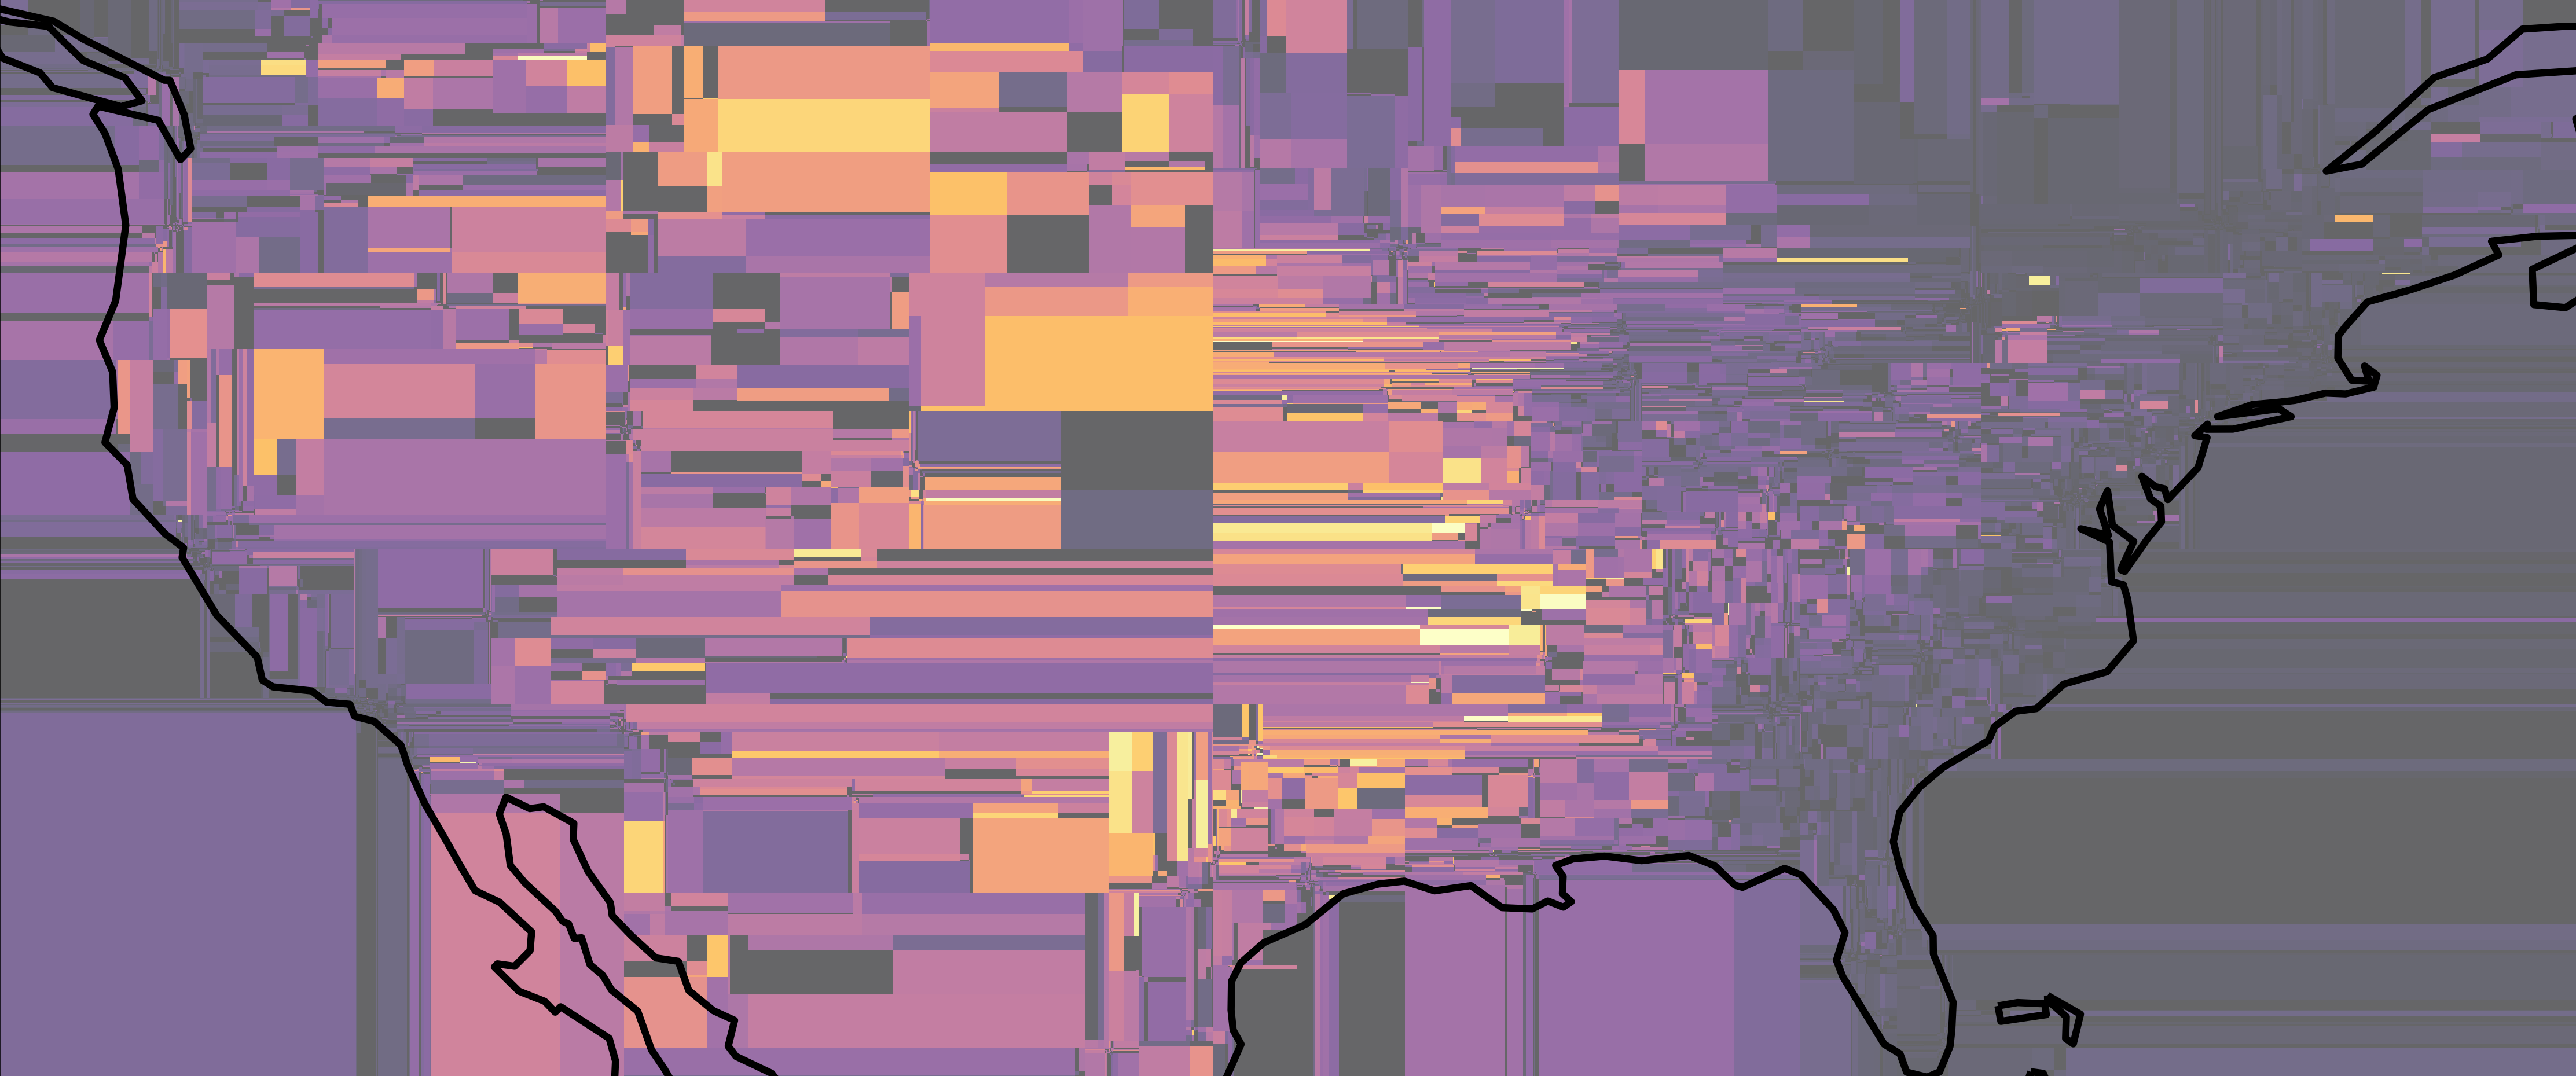
\includegraphics[width=\textwidth]{images/CAIDA_connect_quadplot.png}
    \caption{Ms/km heatmap, quadtree format. Brighter areas indicate higher values.}
    \label{fig:caida_quadplot}
\end{figure}

The smaller the box, the more measurements are in that geographic area. The center of the box is interpreted as a data point and graphed accordingly. Using this technique, the total amount of data points can be reduced from hundreds of thousands to under 1,000, with an average efficiency of about 90\%. This technique was used to generate the heatmap shown in figure \ref{fig:caida_connectivity_heatmap}.
